%!TeX encoding=utf8
\documentclass[ngerman]{scrartcl} 

\newcommand{\authA}{Daniel Scheiermann}
\newcommand{\matA}{3227680}
\newcommand{\authB}{Felix Springer}
\newcommand{\matB}{10002537}
\newcommand{\grpnr}{SLOT}
\newcommand{\Versuchsnummer}{IQ18}
\newcommand{\Versuchsname}{Scanning Laser Optical Tomography}


%%%%%%%%%%%%%%%%%%Capitalized Color - start%%%%%%%%%%%%%%%%%%%%%%%%
\usepackage{xparse}
\usepackage{xcolor}


\ExplSyntaxOn
\NewDocumentCommand{\colorcap}{ O{blue} m }
 {
  \sheljohn_colorcap:nn { #1 } { #2 }
 }

\tl_new:N \l__sheljohn_colorcap_input_tl
\cs_new_protected:Npn \sheljohn_colorcap:nn #1 #2
 {
  % store the string in a variable for usage with \regex_replace_all:nnN
  \tl_set:Nn \l__sheljohn_colorcap_input_tl { #2 }
  \regex_replace_all:nnN
   { ([A-Z]+) } % search a capital letter (or more)
   { \c{textcolor}\cB\{#1\cE\}\cB\{\1\cE\} } % replace the match with \textcolor{#1}{<match>}
   \l__sheljohn_colorcap_input_tl
  \tl_use:N \l__sheljohn_colorcap_input_tl
 }
\ExplSyntaxOff
%%%%%%%%%%%%%%%%%%Capitalized Color - end%%%%%%%%%%%%%%%%%%%%%%%%
%---configure pagelayout
\KOMAoptions{ % read documentation for KOMAScript providing the documentclass scrartcl
DIV=11,
BCOR=0mm,
paper=a4,
fontsize=12pt,
parskip=half,
twoside=false,
titlepage=true
}

%\usepackage[ %Set linespacing
%singlespacing %onehalfspacing,doublespacing
%]{setspace} 

\usepackage[headsepline,footsepline,automark,pagestyleset=KOMA-Script,markcase=ignoreuppercase]{scrlayer-scrpage} %Configure headline and footer

\clearscrheadings
\setlength{\headheight}{3.5\baselineskip}

\ihead[]{\authB~(\matB)\\\authA~(\matA)}
\ohead{
\includegraphics[height=13pt]{IMAGE/luh_logo.png} \\ \Versuchsnummer $ $ \grpnr}

\cfoot{\vspace{-0.75cm}\pagemark}
\pagestyle{scrheadings}

%better positioning of floatings
\renewcommand{\floatpagefraction}{.75} % standard: .5
\renewcommand{\textfraction}{.1} % standard: .2
\renewcommand{\topfraction}{.8} % standard: .7
\renewcommand{\bottomfraction}{.5} % standard: .3
\setcounter{topnumber}{3} % standard: 2
\setcounter{bottomnumber}{2} % standard: 1
\setcounter{totalnumber}{5} % standard: 3

%---Language and umlauts
\usepackage[utf8]{inputenc} %Set UTF-8 encoding, enables ä,ö,ü etc.
\usepackage[ngerman]{babel} %Set document language to ngerman (new german)  
%\usepackage[% improved hyphenation
%expansion=true,
%protrusion=true
%]{microtype}
\usepackage{subcaption}
%\usepackage{subfig} %subcaption includes subfig
%\captionsetup[subfigure]{list=true, font=large, labelfont=bf, 
%labelformat=brace, position=top}

%---Mathmatics (AMS packages )
\usepackage{amsmath} %generell math enviorments e.g. align
\usepackage{amsfonts}
\usepackage{amssymb} 
%\usepackage{amsthm} %math theorems
%\usepackage{upgreek}%provide special form of greek letters e.g. \upmu
\usepackage{float}
%---Units
\usepackage[decimalsymbol=comma]{siunitx}
%\usepackage{units}
%\usepackage[numbers]{natbib}
%\usepackage{pdfpages}
\usepackage{textcomp}
\usepackage{longtable}
%\usepackage{braket}
%\usepackage{color}

%\renewcommand{\arraystretch}{1.2} % Standard-Zeilenhöhe einstellen

%---tables and imgaes
\usepackage{graphicx} %provide \includegraphics[options]{name}
%\usepackage{epstopdf} %enable the use of eps-graphics
\usepackage[hypcap]{caption} %captions out of floating-enviorments(figure,table)
\usepackage{booktabs} %extra lines in tabulars
%\usepackage{flafter} %Place floating-enviorments after references.
%\usepackage[ %
%section %latest ancor for floating-enviorments
%]{placeins}
%\usepackage{verbatim} %long comments \begin{comment} ...\end{comment}

%---Hyperlinks
\usepackage{hyperref} %create table of content and references as links
\hypersetup{
%
%Colors 
colorlinks=true, 
breaklinks=true, 
citecolor=blue, 
linkcolor=black, 
menucolor=red, 
urlcolor=cyan,
%
%pdf-bookmarks
bookmarksopen=false, 
bookmarksopenlevel=0,
% 
%pdf-data
% pdftitle={\titel}, 
% pdfauthor={\writer}, 
% pdfcreator={\writer}, 
% pdfsubject={\titel}, 
% pdfkeywords={\titel} 
%
%misc
plainpages=false,% zur korrekten Erstellung der Bookmarks 
hypertexnames=false,% zur korrekten Erstellung der Bookmarks 
% hyperindex=true,
}


\begin{document}
\title{\Versuchsname $ $ \Versuchsnummer}
\subtitle{Laborpraktikum durchgeführt im Block 1\\
22.10.2018 – 09.11.2018\vspace{1cm}\\ 
\includegraphics[width=.75\linewidth]{IMAGE/luh_logo.png}}
\author{
\authA\\
\matA
\and
\authB\\
\matB
}
\date{\today}

\pagestyle{empty} %Clear headline and footer
\setcounter{page}{0} %Set pagenumber to 0
\maketitle %Create the title

\newpage 

\thispagestyle{empty}
\tableofcontents
\pagestyle{scrheadings}

\setcounter{page}{1}
\newpage


\section{Einleitung}
In diesem Versuch wird die Methode der Tomographie am Beispiel der \colorcap[blue]{Scanning Laser Optical Tomography} - kurz SLOT - untersucht. Dieses ist ein spezielles dreidimensionales Tomographie-Verfahren, das mit Lasern verschiedener Wellenlängen mittels der Ausnutzung von Streuung, Absorption und Fluoreszenz ein bildgebendes Verfahren liefert.\\

Das dreidimensionale Präparat wird ebenenweise durch zweidimensionale Schnitte (Tomogramme) konstruiert und zu einem dreidimensionalen Bildobjekt zusammengesetzt. Das entstandene Bildobjekt ist nun vom Präparat getrennt und virtuell verfügbar. Daraus ergibt sich der Vorteil das Präparat unbeschädigt lassen zu können und dennoch die innere Struktur des Präparates zu untersuchen.\\

\section{Scanning Laser Optical Tomography}
\subsection{Funktionsweise}
SLOT basiert auf einem x-y-Scanner-System mit zwei Silberspiegeln, das den auf die Mitte des Präparates fokussierten Laser abläuft. Das Präparat muss "Aufgeklart" sein, um Streuung beim Übergang zwischen Präparat und Träger des Präparats zu verringern und eine höhere Transmission zu erreichen. Hierzu wird Wasser oder Glycerin genutzt, da dieses einen ähnlichen Brechungsindex wie organische Präparate haben. Das transmittierte Laserlicht wird von einer Photodiode hinter der Probenkammer detektiert. Um eine Rekonstruktion durchführen zu können sind Aufnahmen des Präparats von verschiedenen Richtungen aus nötig, Hintergrund ist die Radontransformation. Diese verschiedenen Aufnahmen werden durch einen Motor ermöglicht der die Kapillare und damit das Präparat dreht. Weiterhin regt das Laserlicht das Präparat zur Fluoreszenz an, welches mittels plankovexen Linsen mit dazwischen liegendem Fluoreszenz-Filter gesammelt und auf den sensitiven Photomuliplier (PMT) geleitet wird.\\

\subsection{Radontransformation}

\section{Versuchsaufbau}

\section{Auflösungsvermögen}

Der Kontrast in Abhängigkeit von der horizontalen und vertikalen Auflösung wurde für verschiedene Fokussierungen, Strahlendurchmesser und Wellenlängen des Lasers gemessen. Dadurch ergibt sich die Modulationsübertragungsfunktion.
 
Bei allen Messungen wurde die Dunkelaufnahme von der normalen abgezogen, um ein Rauschen herauszurechnen.\\

Für geringe Auflösung wurde die Modulationsübertragungsfunktion  in Abhängikeit zur horizontalen Auflösung in Abbildung \ref{fig:Versuch2_Plot2h1} und zur vertikalen Auflösung in Abbildung \ref{fig:Versuch2_Plot2v1} dargestellt.\\
Für hohe Auflösung ist diese zur horizontalen Auflösung in Abbildung \ref{fig:Versuch2_Plot2h2} und zur vertikalen Auflösung in Abbildung \ref{fig:Versuch2_Plot2v2} dargestellt.

Außerdem sind die Modulationsübertragungsfunktionen für hohe Auflösungen in Abbildung \ref{fig:Versuch2_Plot2_all} dargestellt, um diese untereinander besser vergleichen zu können.



\begin{minipage}{\linewidth}
\begin{figure}[H]
	\centering
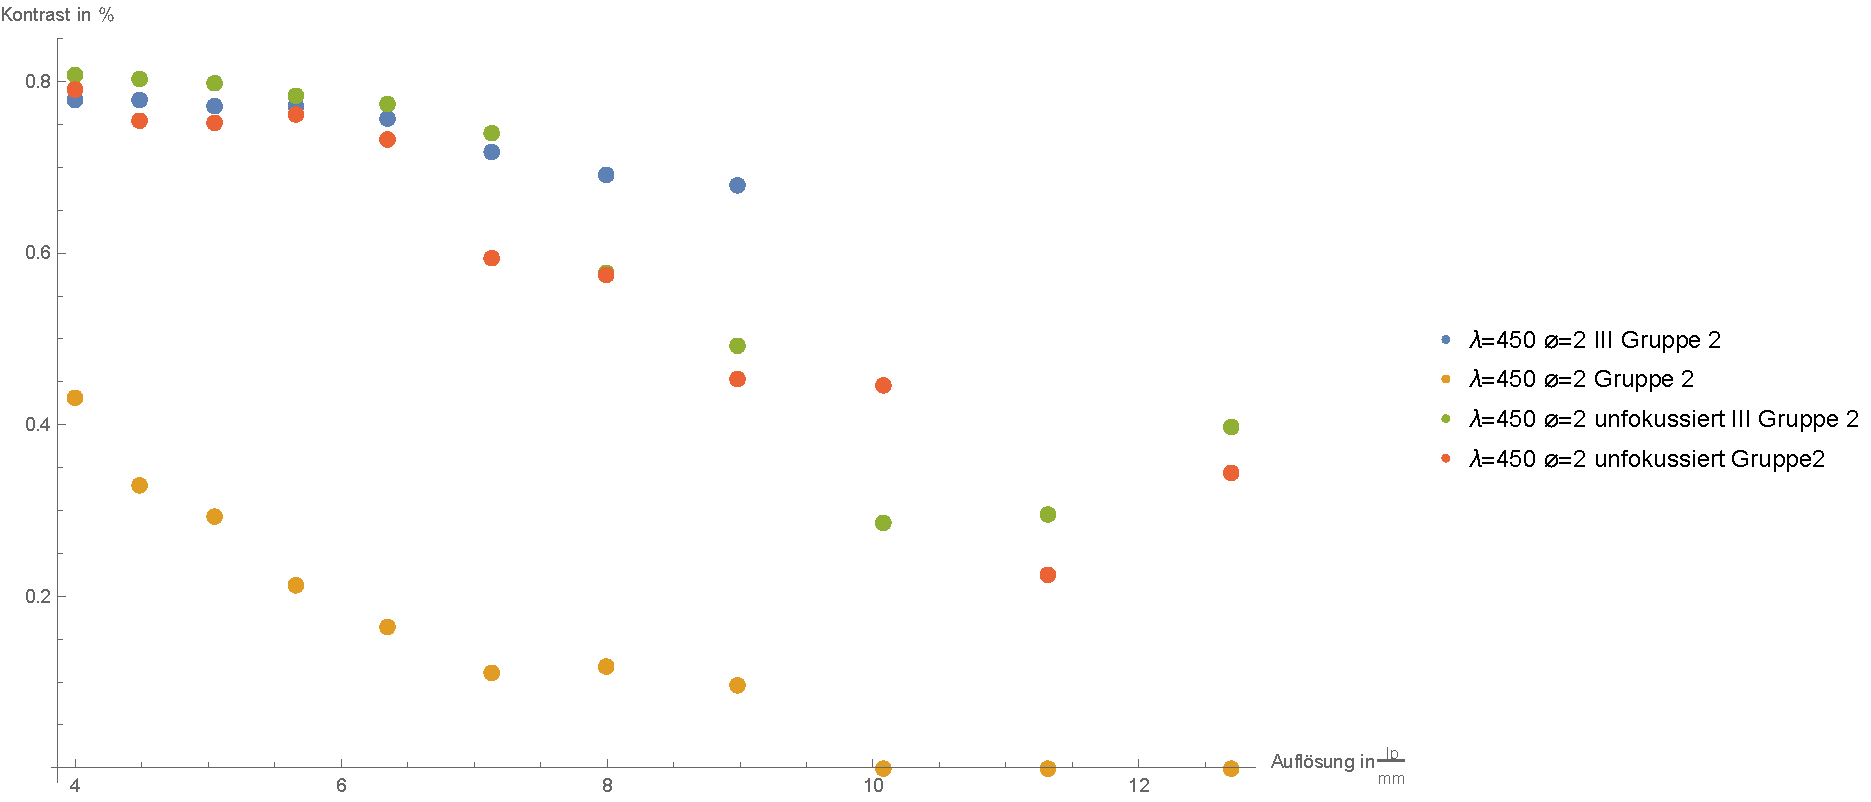
\includegraphics[width=1.0\linewidth]{IMAGE/Versuch2Plot1horizontal2.pdf}
	\caption{Kontrast bei geringer Auflösung (horizontal)}
	\label{fig:Versuch2_Plot2h1}
\end{figure} 

\begin{figure}[H]
	\centering
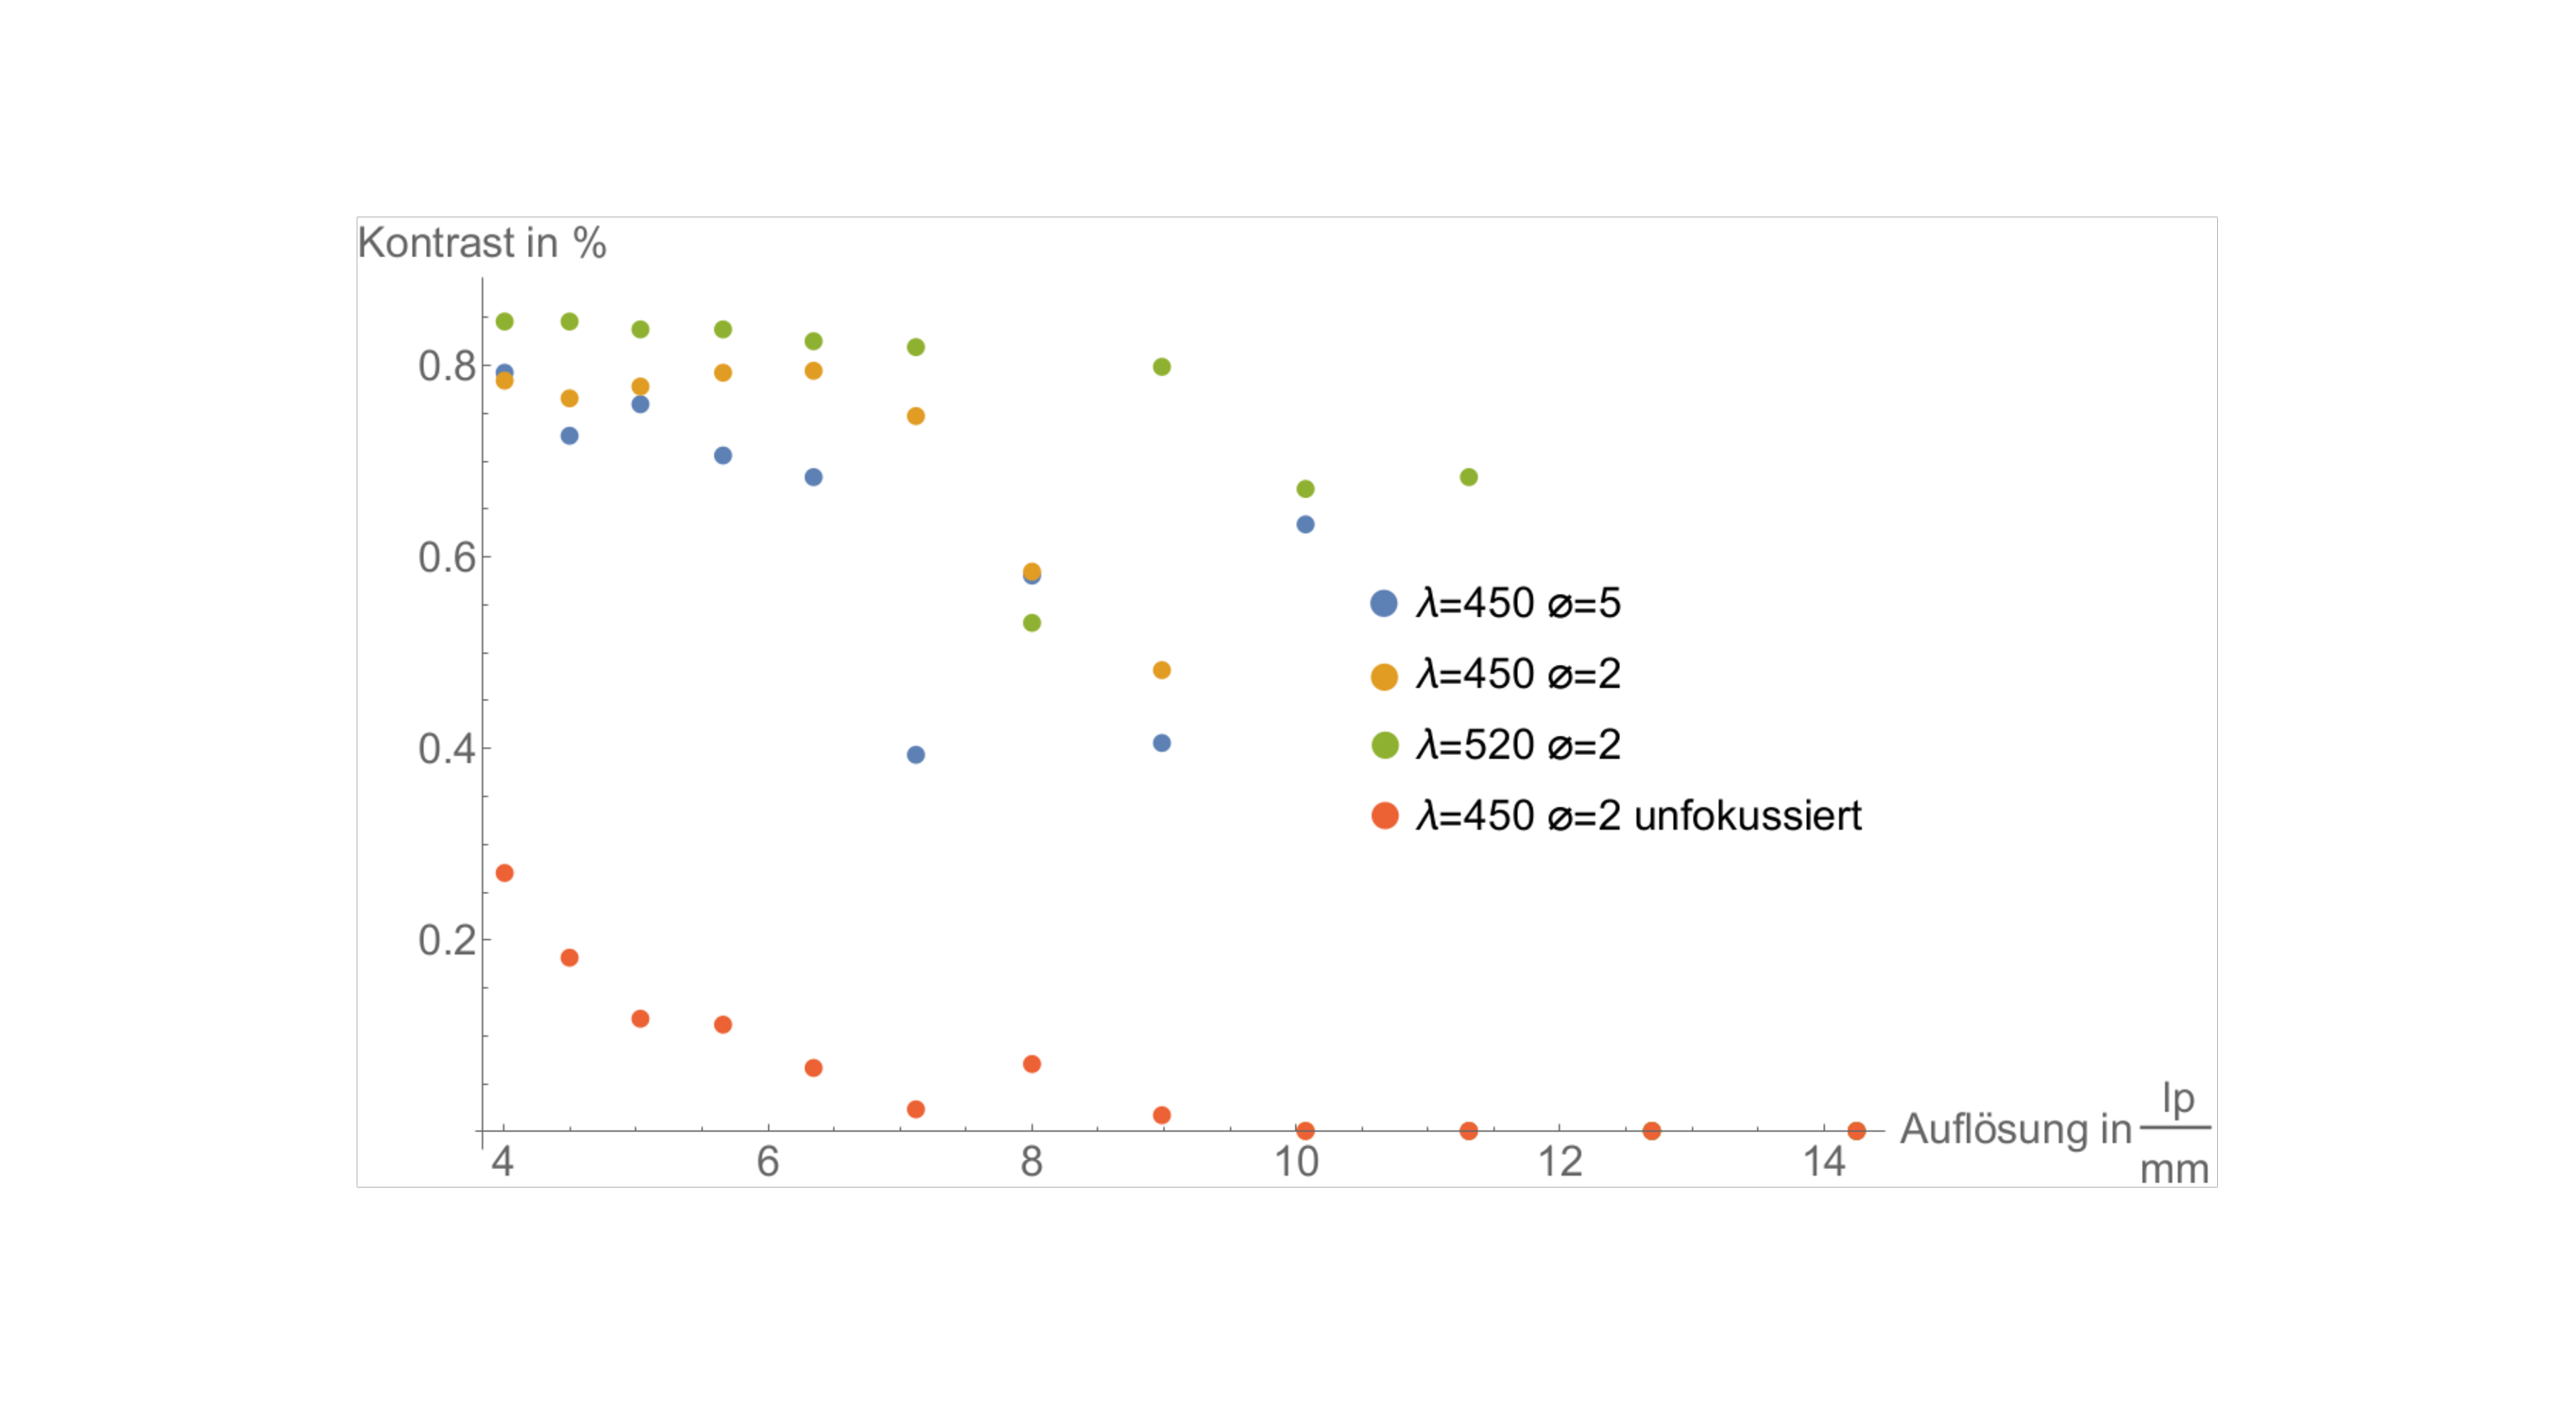
\includegraphics[width=1.0\linewidth]{IMAGE/Versuch2Plot1vertikal2.pdf}
	\caption{Kontrast bei geringer Auflösung (vertikal)}
	\label{fig:Versuch2_Plot2v1}
\end{figure} 

Ein erhöhter Strahlendurchmesser verbessert den Kontrast.\\
Bei geringer Auflösung ist der Kontrast für eine höhere Wellenlänge höher.\\
Der Kontrast ist in horizontaler und vertikaler Richtung von vergleichbarer Höhe.\\
Weiterhin sinkt der Kontrast rapide, falls ohne Fokussierung gemessen wird.

\end{minipage}

\begin{minipage}{\linewidth}
\begin{figure}[H]
	\centering
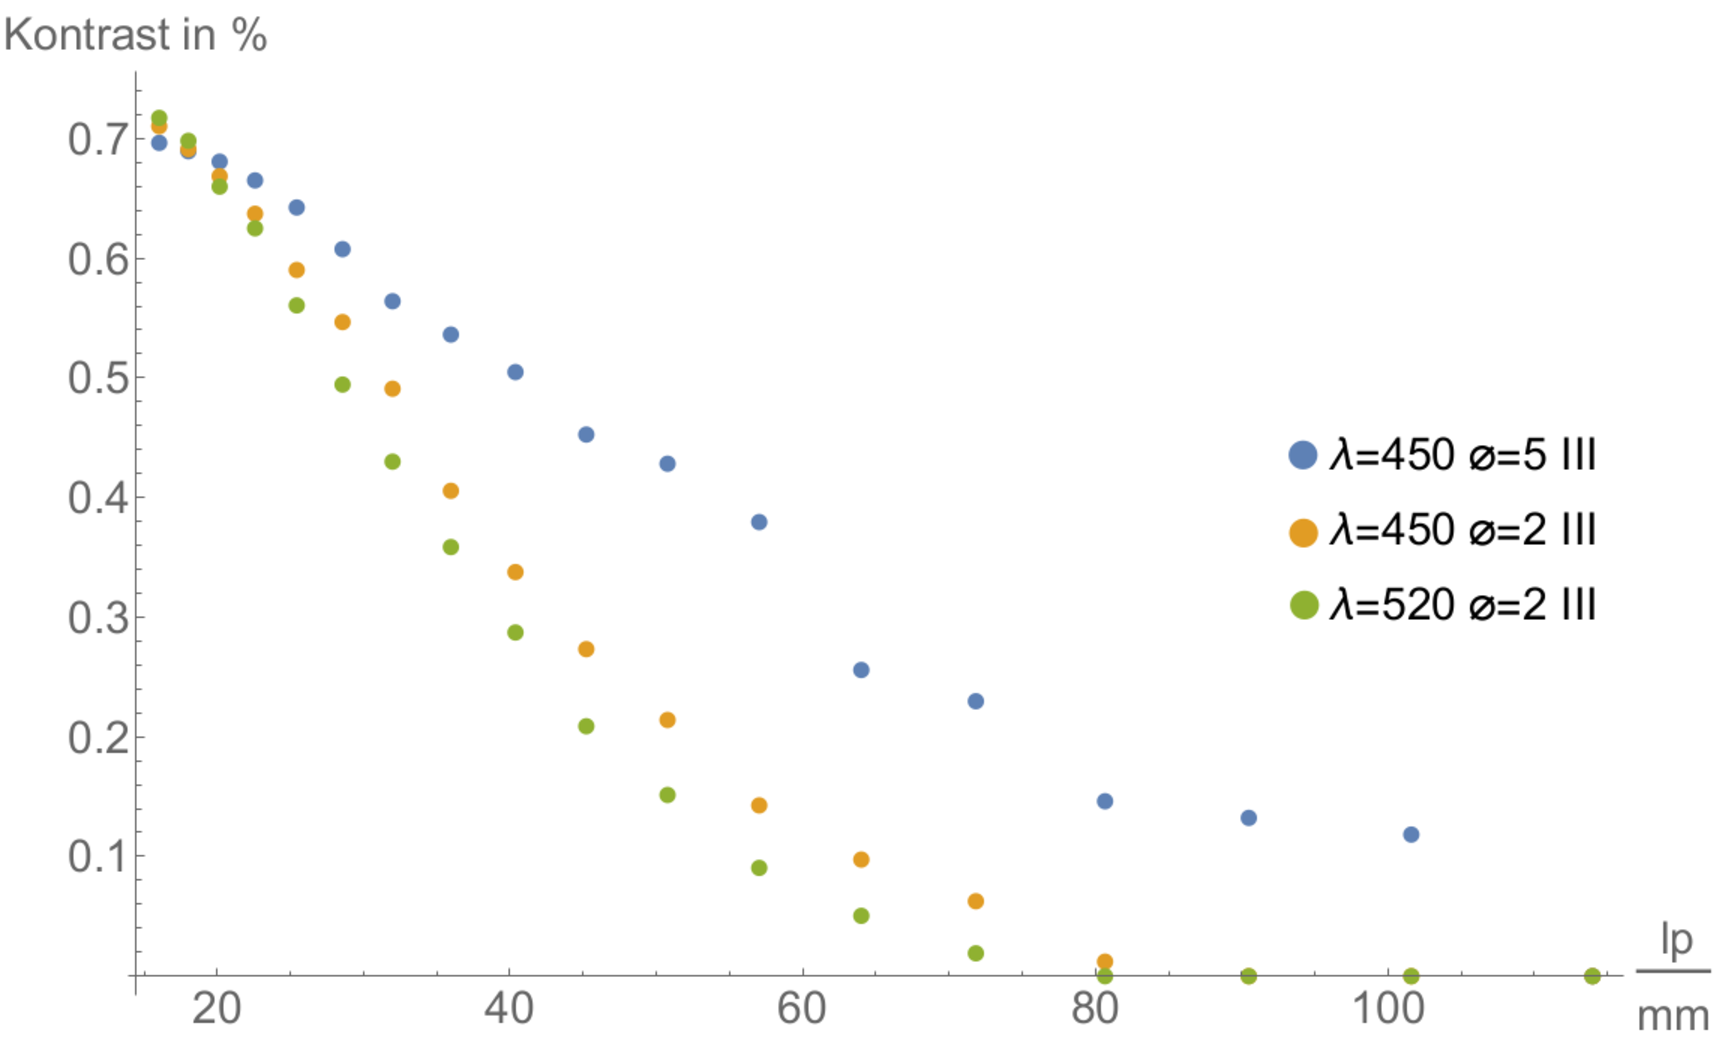
\includegraphics[width=1.0\linewidth]{IMAGE/Versuch2Plot2horizontal2.pdf}
	\caption{Kontrast bei hoher Auflösung (horizontal)}
	\label{fig:Versuch2_Plot2h2}
\end{figure} 

\begin{figure}[H]
	\centering
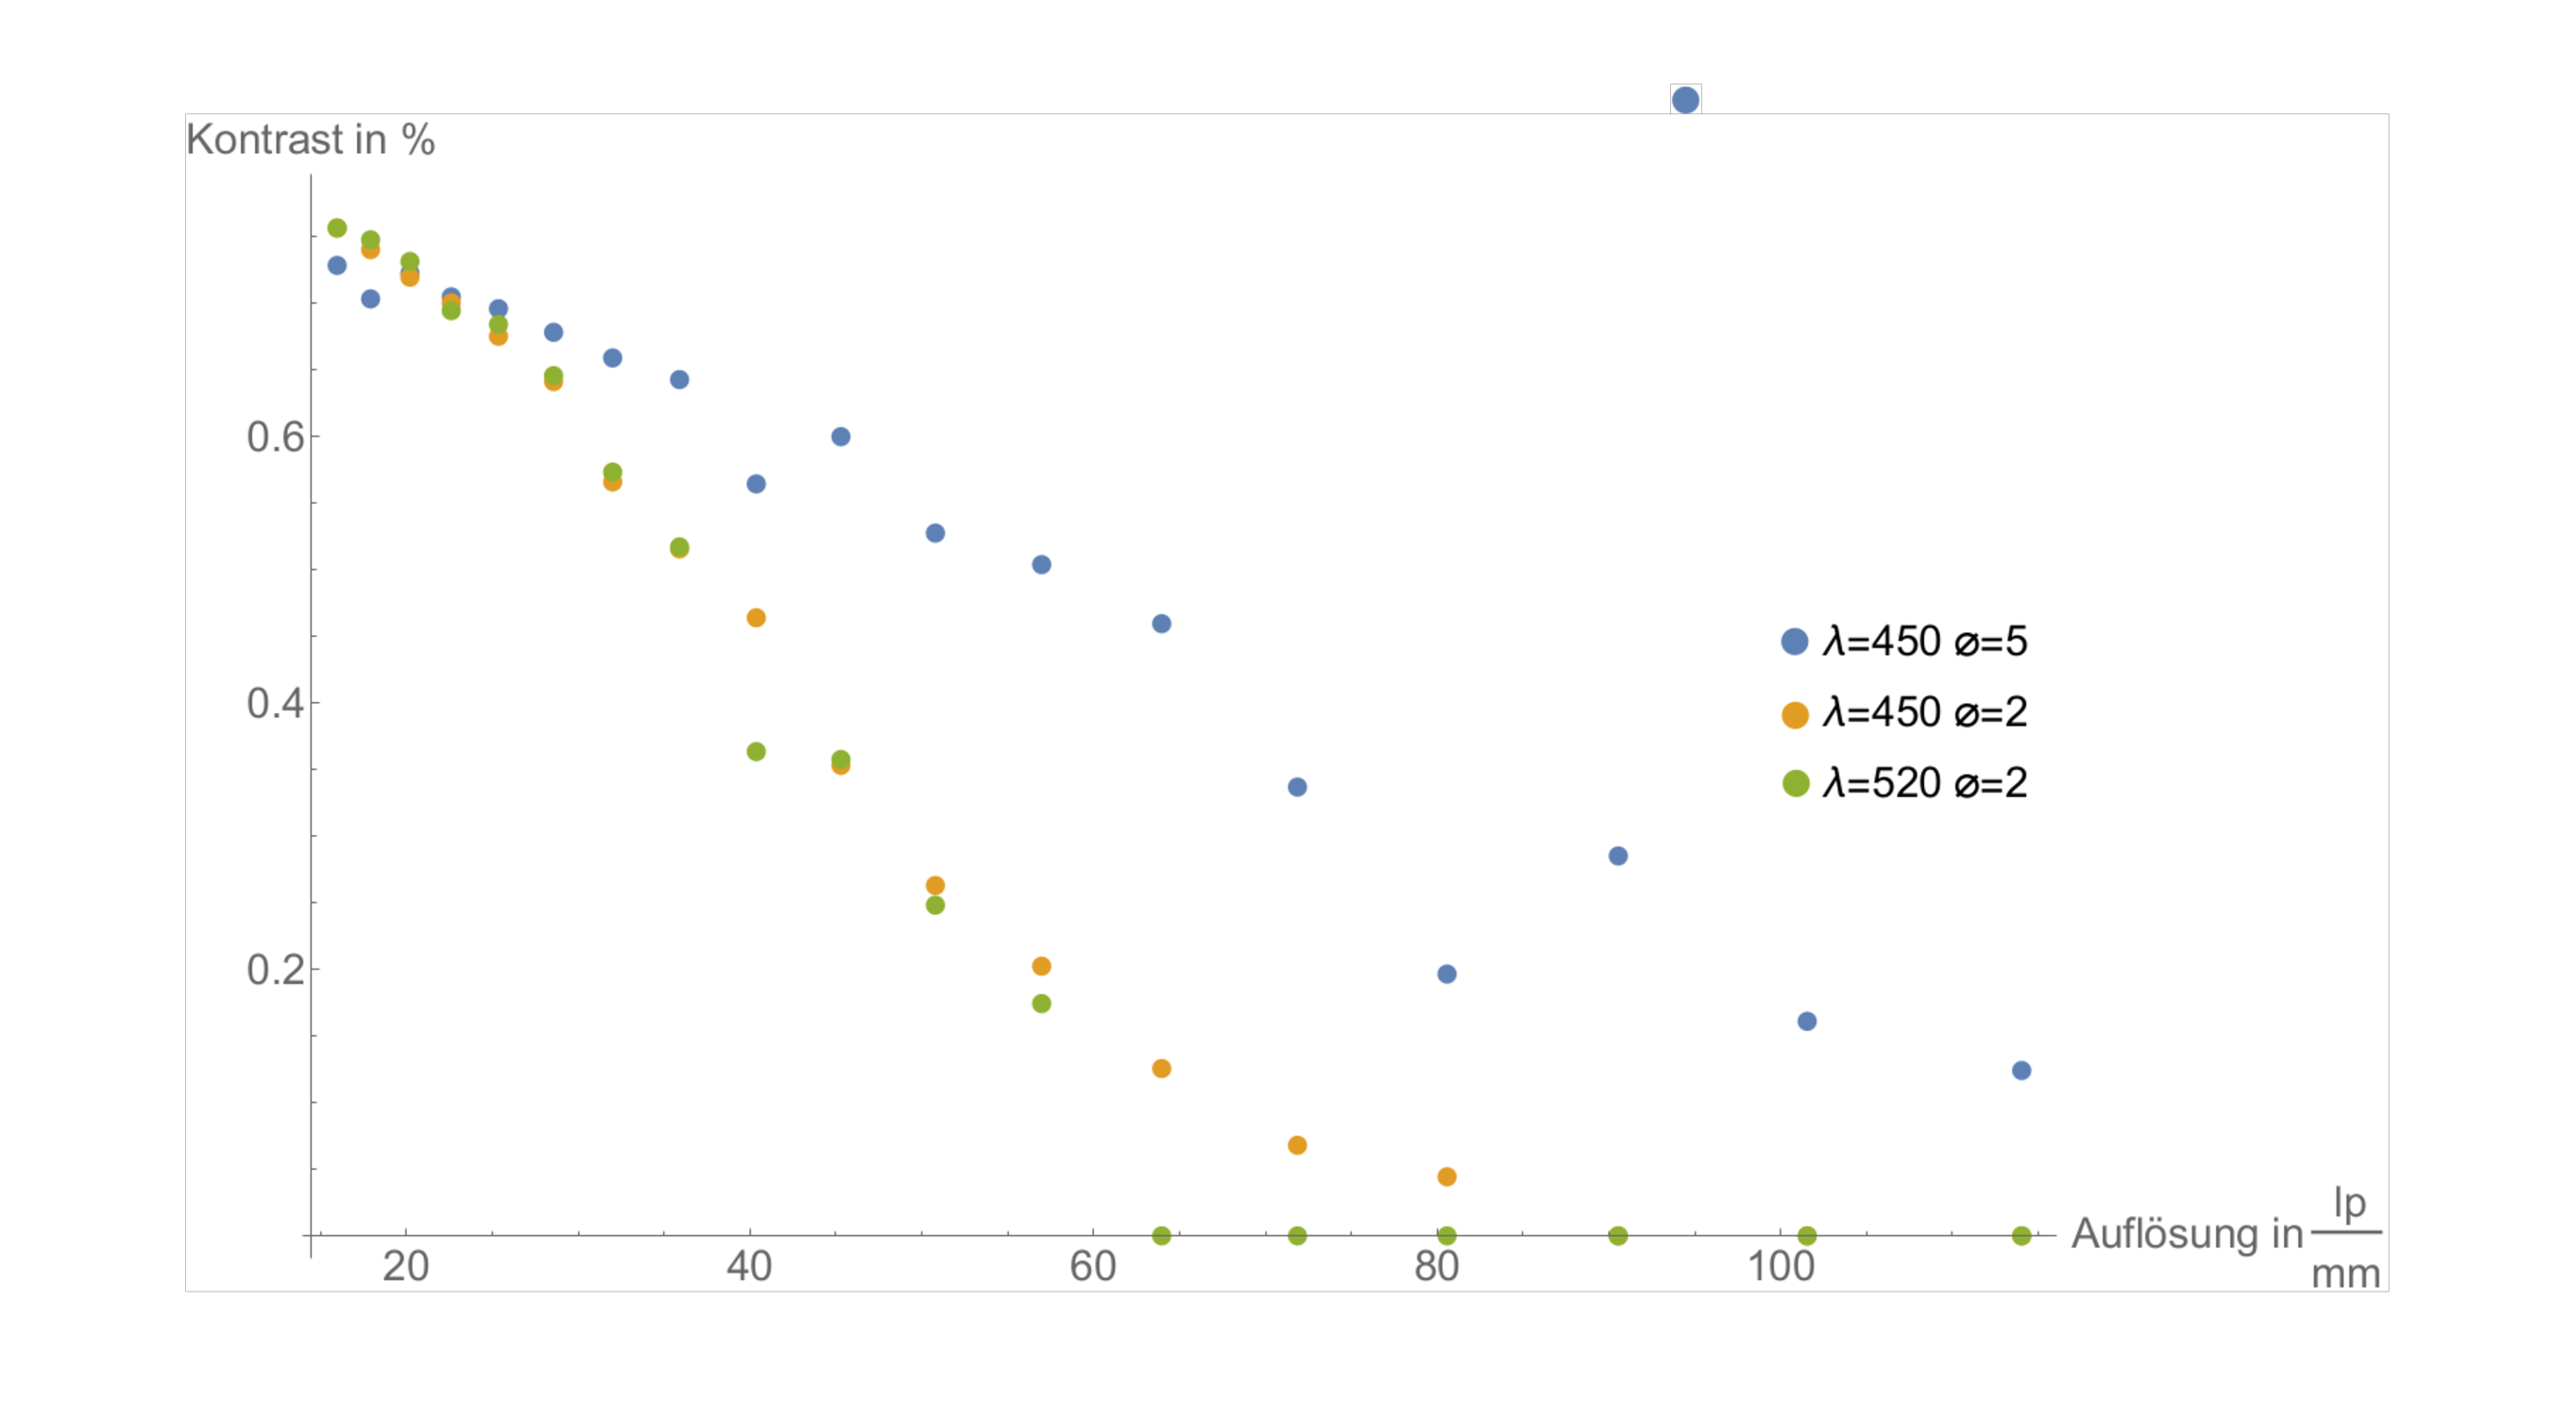
\includegraphics[width=1.0\linewidth]{IMAGE/Versuch2Plot2vertikal2.pdf}
	\caption{Kontrast bei hoher Auflösung (vertikal)}
	\label{fig:Versuch2_Plot2v2}
\end{figure} 

Auch bei hoher Auflösung ist verbessert ein erhöhter Strahlendurchmesser  den Kontrast. Zwar ist der Kontrast bei einer geringen Auflösung bei einer höheren Wellenlänge höher, aber ab etwa einer Auflösung von $20 \frac{lp}{mm}$ erhöht eine kleine Wellenlänge den Kontrast.
\end{minipage}



\begin{figure}[H]
\centering
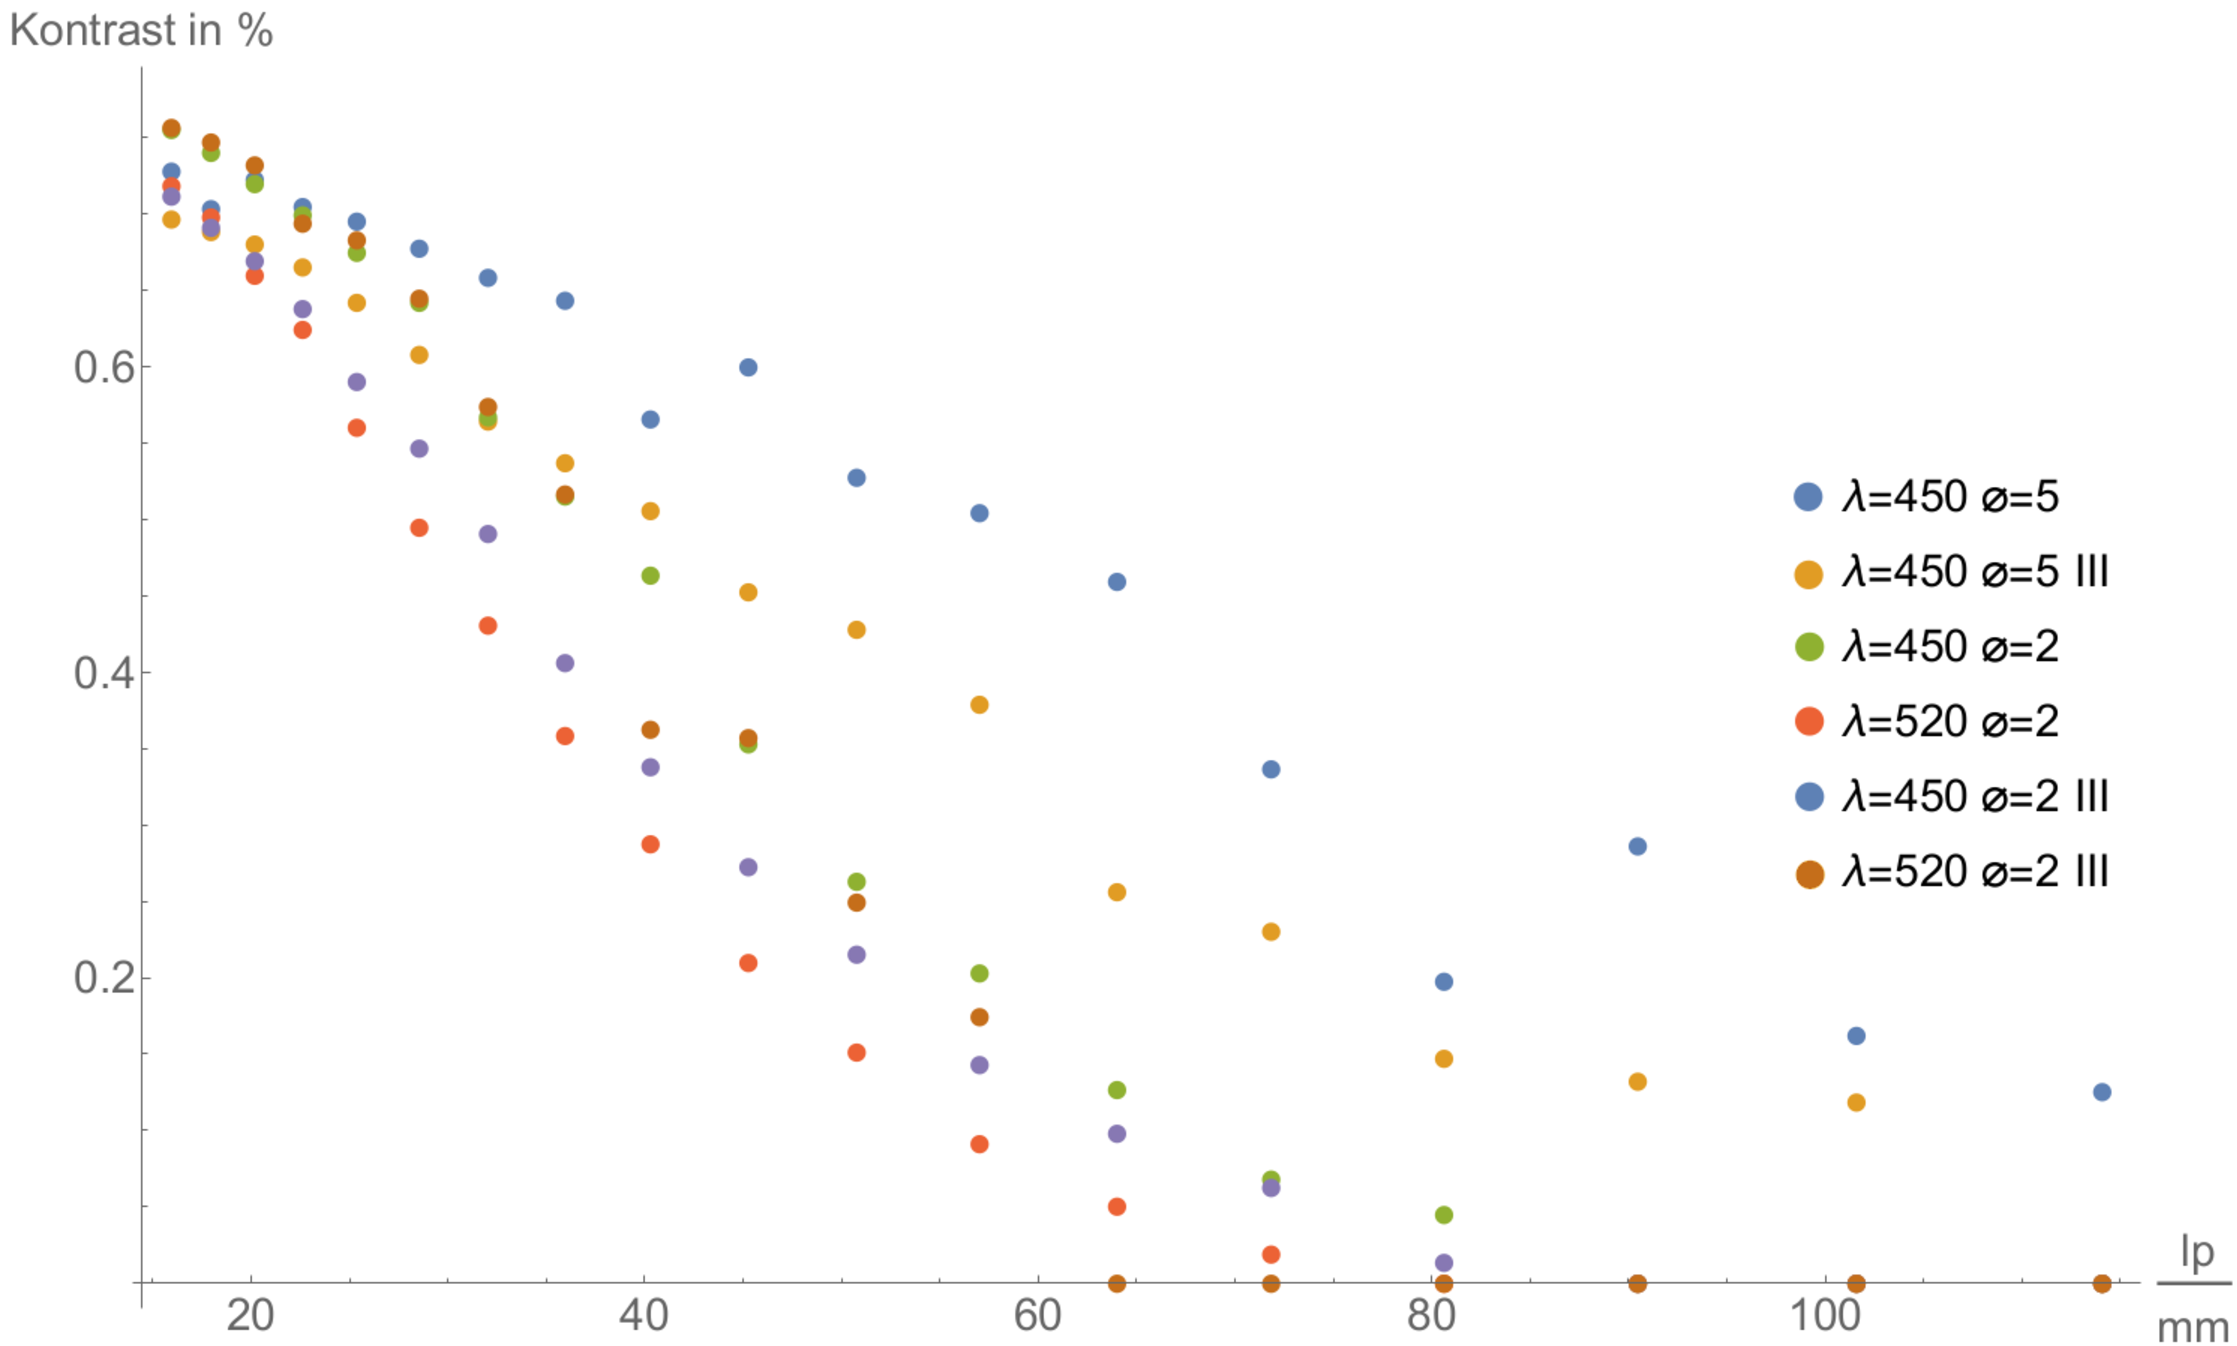
\includegraphics[width=1.0\linewidth]{IMAGE/Versuch2Plot2_all.pdf}
	\caption{Kontrast bei hoher Auflösung (horizontal \& vertikal)}
	\label{fig:Versuch2_Plot2_all}
\end{figure}

%\textcolor{red}{Vielleicht sollte man die Innere mit der Äußeren Aufnahme zusammensetzen und im selben Plot anzeigen, um längere Messkurven zu erhalten.}


%%%%%%%%%%%%%%%%%%%%%%%Ab hier alte Vorlage%%%%%%%%%%%%%%%%%%%%%%%%%%%%%%%%%%%%
\section{Aufnahmen von Heuschreckengehirnen}
In diesem Versuchsabschitt haben wir als Probe ein präpariertes Heuschreckengehirn in den SLOT-Aufbau gestellt.
Die Probe war in einer Küvette und hat sich mit dieser um die $z$-Achse gedreht.
Mit einer 360°-Drehung um die $z$-Achse haben wir also unsere Aufnahmen unter verschieden Einstellungen aufgenommen.
Interessant war bei dieser Messung, dass wir die Fluoreszenz mit dem Photomultiplier (PMT) darstellen konnten, da es sich hier, im Gegensatz zum USAF-Target, um eine 3-dimensionale Probe handelt.

Wichtig für die Auswertung dieser Messung war, dass die Drehachse der Probe nicht präzessiert, was wir leider durch ausporbieren am Aufbau nicht ganz vermeiden konnten.
Die Achse wandert also ca. 4 Pixel von links nach rechts.

Die durchschnitttliche Schieflage $\alpha$  konnten wir bei der Auswertung jedoch ausgleichen.
Dazu haben wir den Drehachsendurchlauf am oberen und unteren Bildrand gemessen und den Winkel $\alpha$ mit
$$\alpha = \arcsin \left( \frac{\Delta{x_{\text{oben}}} - \Delta{x_{\text{unten}}}}{y_{\text{max}}} \right)$$
berechnet.
Hier entspricht $y_\text{max}$ der Anzahl an Pixel auf der $y$-Achse im Bild.

Um $\Delta{x_{\text{oben}}}$ und $\Delta{x_{\text{unten}}}$ messen zu können haben wir die jeweilige Ebene mit 100 verschiedenen $x$-Achsenverschiebungen mit ,,tilt'' rekonstruiert und anschließend das beste Bild herausgesucht (möglichst keine Ringartefakte).

Dann haben wir die Aufnahme mit ,,ImageJ'' um den jeweiligen Winkel gedreht und das Ergebnis wieder mit ,,tilt'' aber dieses mal für alle Ebenen rekonstruiert.
Dabei haben wir auch die mittlere $x$-Achsenverschiebung
$$\Delta{x} = \frac{\Delta{x_{\text{oben}}} - \Delta{x_{\text{unten}}}}{2}$$
beachtet.


Eine Verlängerung der Integrationszeit $\Delta{t}$ von $1 \si{s}$ zu $2 \si{s}$ hatte nur eine Aufhellung des PMT-Bildes zu Folge.
Da wir bei dieser Aufnahme jedoch einen unpassenden Filter verwendeten, zeigt das PMT-Bild auch nur das gestreute Licht. Das Ergebnis ist in Abbildung \ref{fig:lang-int} zu sehen.

\begin{figure}[ht]
\centering
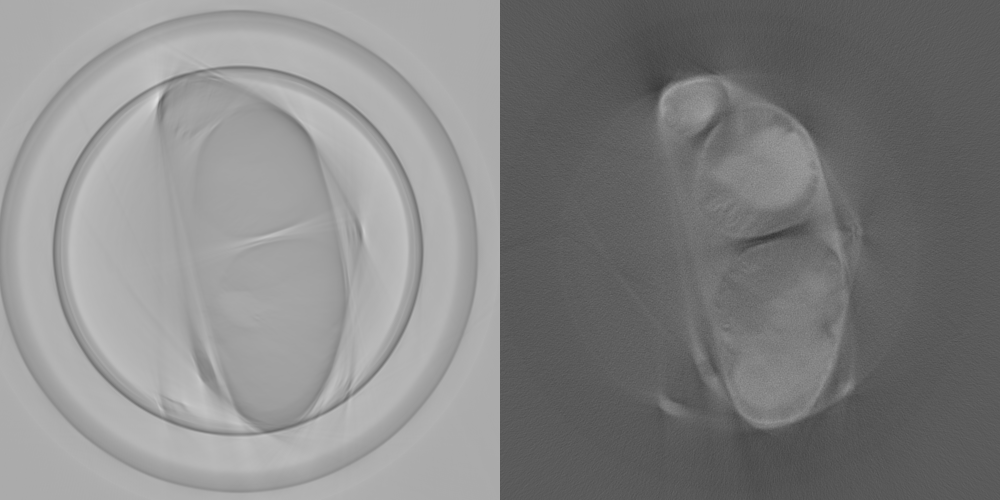
\includegraphics[width=\linewidth]{IMAGE/both-2-450-5-1.png}
\caption{Rekonstruktion: Photodiode links, PMT rechts; $\lambda = 450 \si{nm}$, $\Delta{t} = 2 \si{s}$, $\lambda_\text{Filter} = (520 \pm 36) \si{nm}$, $d_\text{Strahl} = 5 \si{mm}$}
	\label{fig:lang-int}
\end{figure}

Mit der Photodiode lassen sich die äußeren Umrisse gut erkennen, mit dem PMT auch die Dichte im Inneren.

In Abbildung \ref{fig:both-pht} sind 2 Rekonstruktionen der Bilder der Photodiode dargestellt.
Man erkennt, dass das Bild mit der längeren Wellenlänge feinere Strukturen im Heuschreckengehirn darstellt.

\begin{figure}[ht]
\centering
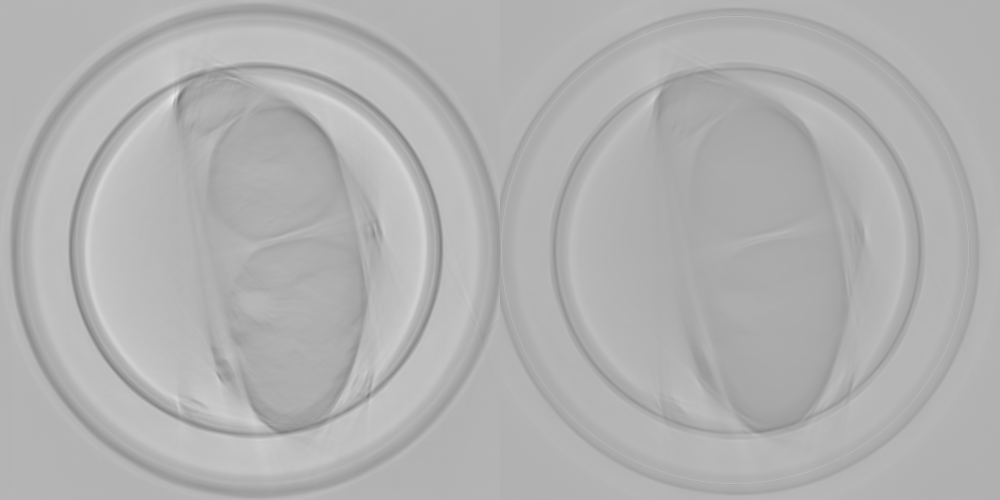
\includegraphics[width=\linewidth]{IMAGE/2-pht.png}
\caption{Rekonstruktion: $\lambda = 520 \si{nm}$ links, $\lambda = 450 \si{nm}$ rechts; Photodiode, $\Delta{t} = 1 \si{s}$, $\lambda_\text{Filter} = (520 \pm 36) \si{nm}$, $d_\text{Strahl} = 5 \si{mm}$}
	\label{fig:both-pht}
\end{figure}

In Abbildung \ref{fig:both-pmt} wurden Bilder des PMT vom jeweiligen Fluoreszenzlicht der Laser rekonstruiert. Im Vergleich stellt man fest, dass man bei $\lambda= 520 \si{nm}$ mehr erkennt.

\begin{figure}[ht]
\centering
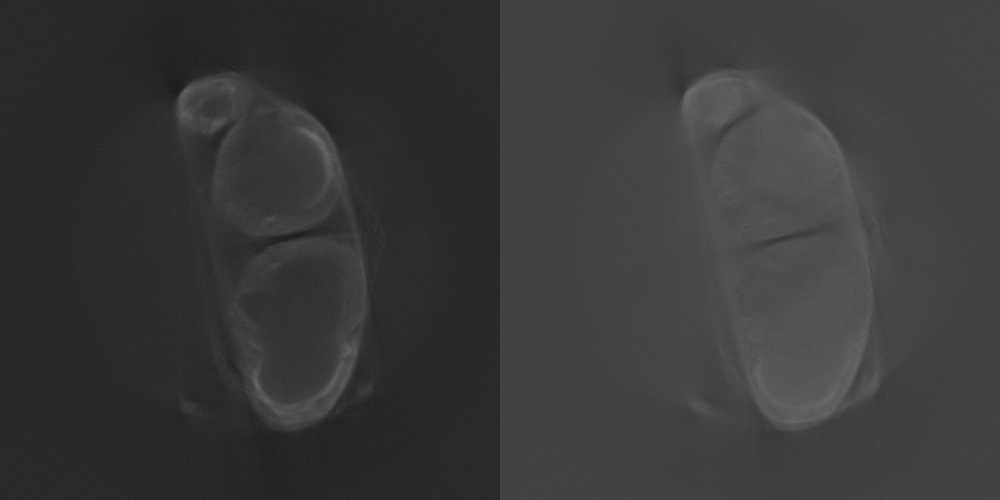
\includegraphics[width=\linewidth]{IMAGE/2-pmt.png}
\caption{Rekonstruktion: $\lambda = 520 \si{nm}$ links mit $\lambda_\text{Filter} = (676 \pm 29) \si{nm}$ links, $\lambda = 450 \si{nm}$ mit $\lambda_\text{Filter} \ge 570 \si{nm}$ rechts; Photodiode, $\Delta{t} = 1 \si{s}$, $d_\text{Strahl} = 5 \si{mm}$}
	\label{fig:both-pmt}
\end{figure}

Mit dem ImageJ-Plugin ,,Volume Viewer'' ist es nach der Rekonstruktion möglich verschiedene Ansichten auf das Heuschreckengehirn zu generieren. Ein anschauliches Beispiel ist in Abbildung \ref{fig:3d} zu finden.

\begin{figure}[ht]
\centering
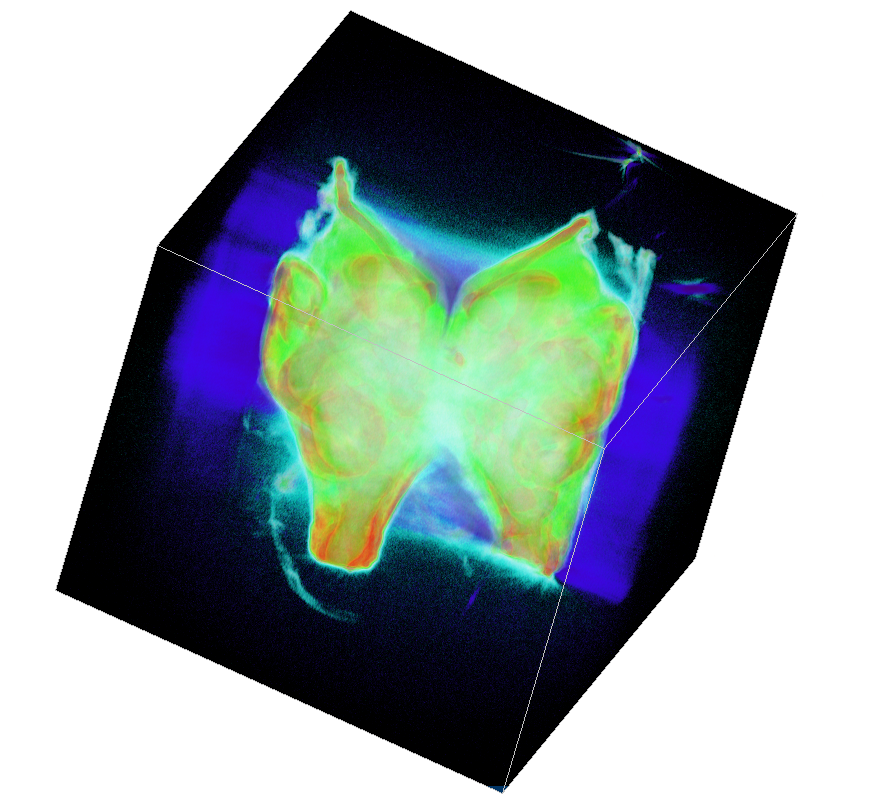
\includegraphics[width=\linewidth]{IMAGE/3dtomo.png}
\caption{3-dimensionale Ansicht einer PMT-Aufnahme: $\lambda = 520 \si{nm}$ mit $\lambda_\text{Filter} = (676 \pm 29) \si{nm}$, $\Delta{t} = 1 \si{s}$, $d_\text{Strahl} = 5 \si{mm}$}
	\label{fig:3d}
\end{figure}


%\clearpage
%\begin{thebibliography}{99}
%	\bibitem{Schaltung1} \textsc{Saure aus Wikimedia Commons}, \emph{Gleichrichter-Schaltung mit Glättung} (26. August 2009) (Stand: 08.03.2018) \url{https://commons.wikimedia.org/w/index.php?title=File:Gleichrichter-Schaltung.svg&oldid=291347227&uselang=de}
%\end{thebibliography}

\end{document}
